\documentclass[border=5pt]{standalone}
\usepackage{tikz}
\usetikzlibrary{calc, positioning}
\usepackage{amsmath}
\begin{document}
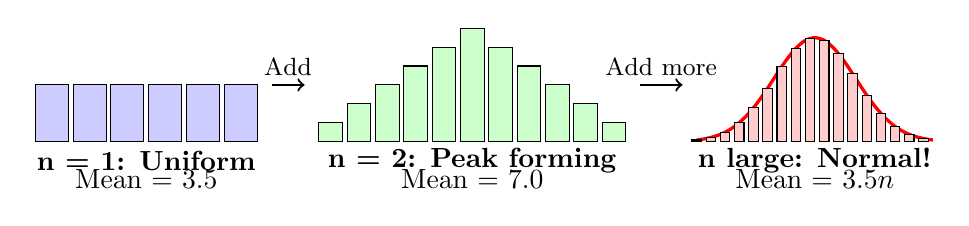
\begin{tikzpicture}[scale=0.6]
% n=1 (Uniform distribution)
\draw[fill=blue!20, draw=black] (0,0) rectangle (0.7,1.2);
\draw[fill=blue!20, draw=black] (0.8,0) rectangle (1.5,1.2);
\draw[fill=blue!20, draw=black] (1.6,0) rectangle (2.3,1.2);
\draw[fill=blue!20, draw=black] (2.4,0) rectangle (3.1,1.2);
\draw[fill=blue!20, draw=black] (3.2,0) rectangle (3.9,1.2);
\draw[fill=blue!20, draw=black] (4.0,0) rectangle (4.7,1.2);
\node at (2.35, -0.4) {\textbf{n = 1: Uniform}};
\node at (2.35, -0.8) {Mean = 3.5};

% n=2 (Triangular-like)
\draw[fill=green!20, draw=black] (6,0) rectangle (6.5,0.4);
\draw[fill=green!20, draw=black] (6.6,0) rectangle (7.1,0.8);
\draw[fill=green!20, draw=black] (7.2,0) rectangle (7.7,1.2);
\draw[fill=green!20, draw=black] (7.8,0) rectangle (8.3,1.6);
\draw[fill=green!20, draw=black] (8.4,0) rectangle (8.9,2.0);
\draw[fill=green!20, draw=black] (9.0,0) rectangle (9.5,2.4);
\draw[fill=green!20, draw=black] (9.6,0) rectangle (10.1,2.0);
\draw[fill=green!20, draw=black] (10.2,0) rectangle (10.7,1.6);
\draw[fill=green!20, draw=black] (10.8,0) rectangle (11.3,1.2);
\draw[fill=green!20, draw=black] (11.4,0) rectangle (11.9,0.8);
\draw[fill=green!20, draw=black] (12.0,0) rectangle (12.5,0.4);
\node at (9.25, -0.4) {\textbf{n = 2: Peak forming}};
\node at (9.25, -0.8) {Mean = 7.0};

% n=large (Bell-shaped)
\draw[red, very thick] plot[smooth, domain=0:5] (14+\x, {2.2*exp(-(\x-2.5)^2/1.5)});
\foreach \x in {0,0.3,...,5} {
    \pgfmathsetmacro{\height}{2.2*exp(-(\x-2.5)^2/1.5)}
    \draw[fill=red!20, draw=black] (14+\x-0.1,0) rectangle (14+\x+0.1,\height);
}
\node at (16.5, -0.4) {\textbf{n large: Normal!}};
\node at (16.5, -0.8) {Mean = $3.5n$};

% Arrows
\draw[thick, ->] (5, 1.2) -- (5.7, 1.2);
\draw[thick, ->] (12.8, 1.2) -- (13.7, 1.2);
\node[above] at (5.35, 1.2) {\small Add};
\node[above] at (13.25, 1.2) {\small Add more};
\end{tikzpicture}
\end{document}
